\section{Solutions}

%N, P accumulation ability
\begin{frame}{N, P accumulation ability}
\begin{figure}
	\centering
	\begin{columns}[T]
	\column{0.5\textwidth}
	\subfigure{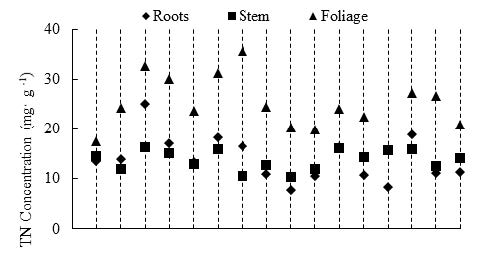
\includegraphics[width=\textwidth,height=0.3\textheight]{TN-p.jpg}}
	\subfigure{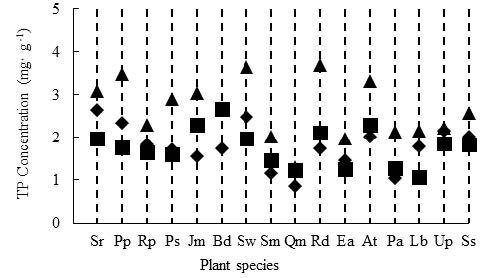
\includegraphics[width=\textwidth,height=0.3\textheight]{TP-p.jpg}}	
	%	\column{{0.01\textwidth}}
	\column{0.5\textwidth}
	\subfigure{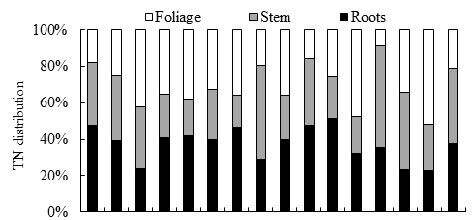
\includegraphics[width=\textwidth,height=0.3\textheight]{TN.jpg}}
	\subfigure{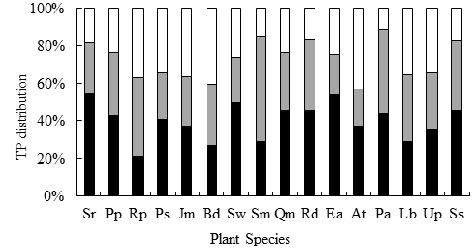
\includegraphics[width=\textwidth,height=0.3\textheight]{TP.jpg}}	
\end{columns}
\caption{Concentration and distribution of total nitrogen (TP) and total phosphorus (TP) in plants. \cite{yu2014biomass}}
%Syringa reticulate (Sr), Prunus padus (Pp), Robinia pseudoacacia (Rp), Pterocarya stenoptera (Ps), Juglans mandshuriea (Jm), Berberis dielsiana (Bd), Sambucus williamsii, Salix matsudana (Sm), Quercus mongolica (Qm), Rosa davurica (Rd), Euonymus alatus (Ea), Acer truncatum (At), Populus alba (Pa), Lespedeza bicolor (Lb), Ulmus pumila (Up) and Sorbaria sorbifolia (Ss). 

\end{figure}
\end{frame}

%Effects of stand structure on biodiversity and water-holding capacity
\begin{frame}{Effects of stand structure on species diversity and water-holding capacity}
\begin{table}
	\caption{Effects of stand structure on species diversity and water-holding capacity}
%	\begin{tabular}{@{}l@{}|@{}c@{}c@{}c@{}c@{}c@{}c@{}|@{}c@{}c@{}}
	\begin{tabular}{@{}l@{}|@{}cccccc@{}|@{}cc@{}}
		\toprule
		\multirow[c]{3}{4ex}{Treat\\ment} & \multicolumn{6}{c}{Species number} & \multicolumn{2}{|c}{Water}\\
		&\multicolumn{3}{c}{First year} & \multicolumn{3}{c}{Second year}& \multicolumn{2}{|c}{storage ($t/hm^2$)}\\
		& Herb&Shrub & Tree &Herb&Shrub & Tree&Total& Non-capillary\\
		\midrule
		CK&3&7&14&3&7&15&1022&220\\
		Weak&3&7&15&3&8&16&1054&260\\
		Medium&4&8&16&4&8&18&1085&295\\
		Intense&4&8&18&5&10&20&1100&324\\
		\bottomrule
	\end{tabular}
\end{table}
\end{frame}